\documentclass{article}
\usepackage[utf8]{inputenc}
\usepackage[polish]{babel}
\usepackage[T1]{fontenc}
\usepackage{graphicx}
\usepackage{tabto}
\usepackage{pgfplots}







\title{Spadek swobodny}
\author{Mateusz Głuchowski}
\date{December 2022}

\begin{document}

\maketitle

\section{Wprowadzenie teoretyczne}
\begin{flushleft}
    Spadek swobodny jest definiowany jako ruch odbywający się pod wpływem ciężaru bez oporów ośrodka.
\end{flushleft}

\begin{flushleft}
    
    Jeżeli spadek spełnia warunki takie jak:\\
        \> •	ma miejsce z małej wysokości w pobliżu Ziemi\\
        \> •	dotyczy ciała o stosunkowo dużej gęstości\\
        \> •	ciało posiada aerodynamiczny kształt,\\

\end{flushleft}

\begin{flushleft}
    wówczas można ruch takiego ciała traktować z przybliżeniem jako ruch jednostajnie przyspieszony z przyspieszeniem ziemskim nieposiadającym prędkości początkowej. W tym przypadku ruch ten opisuje kinetyczne równianie ruchu:

    \begin{equation}
        h_{(t)} = h_{0} - \frac{g*t^{2}}{2}
    \end{equation}

    gdzie: \\
    \> $h_{(t)}$ - wysokość na jakiej znajduje się ciało po czasie t \\ 
    \> $h_{0}$ - początkowa wysokość ciała (wysokość z jakiej spada ciało)\\
    \> $t$ - czas spadania ciała \\
    \> $g$ - przyspieszenie ziemskie ($9,81 \frac{m}{s^{2}}$)\\
    
\end{flushleft}

\begin{flushleft}
    W spadku swobodnym czas spadania ciała oznacza się wzorem:
    \begin{equation}
    t = \sqrt{\frac{2*h}{g}}
    \end{equation}

    gdzie: \\
    \> $t$ - czas spadania ciała\\
    \> $h$ - wysokość\\
    \> $g$ - przyspieszenie ziemskie ($9.81 \frac{m}{s^{2}}$) \\
    
\end{flushleft}

\section{Przebieg eskperymentu}


\begin{center}
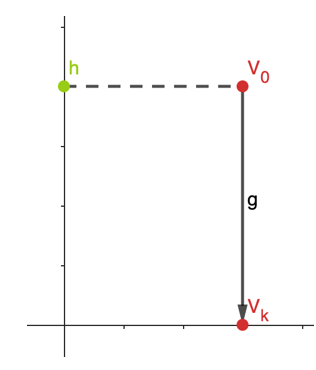
\includegraphics[scale=1.0]{1.png}


Rys. 1
\end{center}

\begin{flushleft}
    Na schemacie przedstawionym powyżej widnieje ciało znajdujące się ciało na wysokość $h$ z prędkością początkową $v_{0} = 0$. Ciało porusza się z ruchem jednostajnie przyspieszonym pionowo w dół, zgodnie z wektorem $\vec{g}$. Przyspieszeniem $a = 9,81 {m/s^2} (a = g = 9,81 m/s^2)$. Swoją podróż ciało kończy przy uderzeniu w powierznie z prędkością $v_{k}.$
\end{flushleft}
\section{Wyniki pomiarów}

    Wykres przedstawia wyniki pomiarów z zestawieniem czasu w stosunku do przebytej drogi. Jest to zwizualizowanie ruchu jednostajnie przyspieszonego: 

\begin{tikzpicture}
\begin{axis}[
    title={Stosunek czasu do przebytej drogi w spadku swobodnym},
    xlabel={$t[m]$},
    ylabel={$s[m]$},
    xmin=0, xmax=10,
    ymin=0, ymax=500,
    xtick={0, 1, 2, 3, 4, 5, 6, 7, 8, 9, 10},
    ytick={0,100, 200, 300, 400, 500},
    ymajorgrids=true,
    grid style=dashed,
    enlargelimits=false,
]


\addplot[
    mesh,
    samples=100,
    domain=-10:10,
    color=red,
    size=1.7pt,
]
{(9.81*x^2)/2};

\addplot+[
    only marks, 
    mark size=0.5pt,
    color=blue,
]
table[meta=s]
{Zeszyt1.csv};


 \legend{$(g*t^2)/2$}
 
\end{axis}
\end{tikzpicture}


\section{Wnioski:}
         •	W przypadku spadku swobodnego, który odbywa się blisko powierzchni Ziemi, gdy ciało charakteryzuje się dużą gęstością, można pominąć siłę oporu jaką jest opór powietrza.\\
         •	Spadek swobodny jest to ruch jednostajnie przyspieszony co widać na wykresie, gdy wartości czasu i drogi wzrastają.\\
        •	Spadek swobodny odbywa się jedynie przy wykorzystaniu siły przyciągania ziemskiego (siły grawitacji).\\



\end{document}
